\documentclass[aspectratio=169, table, 12pt]{beamer}

\usepackage{colortbl}
\usepackage{xcolor}
\usepackage{listings}
\usepackage{tabularx}
\usepackage{tikz}
\usetikzlibrary{arrows.meta, positioning, calc, fit, shapes.geometric}

\makeatletter
\def\input@path{{../theme/}}
\makeatother
\graphicspath{{../theme/}{../../figures/}}
\usetheme{Pradita}

\definecolor{praditagreen}{RGB}{37, 113, 71}

% Tema membuat garis tabel berwarna putih. Dikembalikan agar tabel terbaca.
\arrayrulecolor{black}
\setlength{\arrayrulewidth}{0.5pt}

% Kolom X rata kiri, dipakai pada tabel dengan kolom X yang sempit, agar
% spasi antarkata tidak meregang.
\newcolumntype{Y}{>{\raggedright\arraybackslash}X}

\lstdefinelanguage{bash}{
  keywords={},
  basicstyle=\ttfamily\scriptsize,
  ndkeywords={cd, curl, python, python3, tail},
  ndkeywordstyle=\color{purple}\bfseries,
  sensitive=true,
  commentstyle=\color{gray},
  numbers=none,
  breaklines=true,
  frame=lines,
  backgroundcolor=\color{lightgray!10},
  tabsize=2,
  comment=[l]{\#},
  showstringspaces=false
}

% Gaya Python disamakan dengan naskah bab, tanpa nomor baris.
\lstdefinestyle{PythonStyle}{
  language=Python,
  basicstyle=\ttfamily\scriptsize,
  morekeywords={with, as, yield, async, await, match, case},
  keywordstyle=\color{blue}\bfseries,
  emph={queue, json, antrean},
  emphstyle=\color{purple}\bfseries,
  commentstyle=\color{gray}\itshape,
  stringstyle=\color{red},
  numbers=none,
  breaklines=true,
  frame=lines,
  backgroundcolor=\color{lightgray!10},
  tabsize=2,
  showstringspaces=false
}

\title{\Huge Sistem Real-Time\\ \vspace{10pt} dan Asinkron}
\subtitle{IF140303 - Pengembangan Aplikasi Web}
\author{\textbf{Alfa Yohannis}}

\begin{document}

\frame{\titlepage}

\begin{frame}[fragile]
  \frametitle{Isi Pertemuan}
  \vspace{14pt}
  \begin{columns}[t]
    \column{0.5\textwidth}
    {\small\tableofcontents[sections={1-7}]}

    \column{0.5\textwidth}
    {\small\tableofcontents[sections={8-13}]}
  \end{columns}
\end{frame}

\begin{frame}{\hfill}
  \centering
  \Huge{\textbf{Siapa yang berbicara lebih dahulu,\\server atau klien?}}
\end{frame}

\section{Tujuan dan Kerangka Bahasan}

\begin{frame}{\hfill}
  \centering
  \Huge{\textbf{Tujuan dan Kerangka Bahasan}}
\end{frame}

\begin{frame}{{\Large Tujuan Pembelajaran}}
  \vspace{10pt}
  \begin{itemize}
    \item Mengukur keterlambatan dan biaya \textit{polling}, SSE, serta
          WebSocket pada peristiwa yang sama.
    \item Merancang alur asinkron memakai antrean, \textit{worker}, dan
          \textit{webhook}, lalu menunjukkan jeda \textit{retry}-nya pada
          hasil pengukuran.
    \item Membedakan pengiriman \textit{at-least-once} dari sekali saja, lalu
          membuktikan \textit{consumer} idempoten menahan duplikatnya.
  \end{itemize}
\end{frame}

\begin{frame}{{\Large Dua Kebutuhan yang Sering Disatukan}}
  \vspace{12pt}
  \begin{itemize}
    \item Pengguna ingin melihat perubahan segera, tanpa menekan
          \textit{refresh}. Ini menuntut jalan dari server ke klien, padahal
          HTTP dirancang untuk arah sebaliknya.
    \item Pekerjaan yang lama tidak boleh menahan jawaban. Ini menuntut
          pekerjaan hidup lebih lama daripada permintaan yang memulainya.
  \end{itemize}
  \vspace{10pt}
  {\small Demonya dua bagian: satu server peristiwa dengan tiga cara
  pengiriman, dan satu alur asinkron berisi antrean, \textit{worker}, serta
  penerima \textit{webhook}.}
\end{frame}

\section{Polling, SSE, dan WebSocket}

\begin{frame}{\hfill}
  \centering
  \Huge{\textbf{Polling, SSE, dan WebSocket}}
\end{frame}

\begin{frame}{{\Large Tiga Cara Membawa Peristiwa ke Klien}}
  \vspace{4pt}
  \centering
  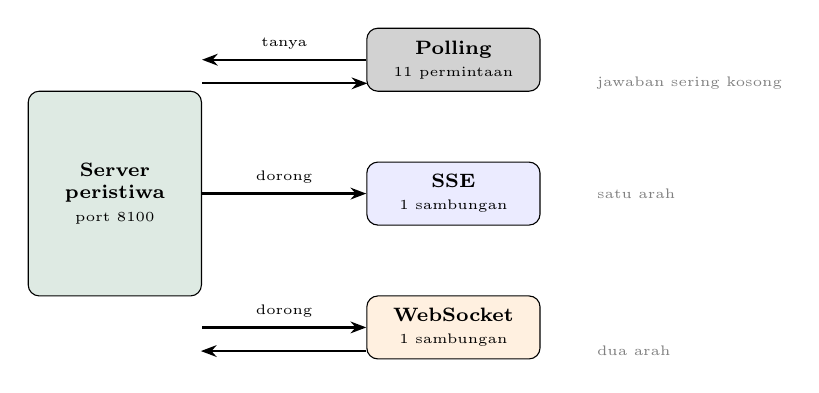
\begin{tikzpicture}[
    font=\scriptsize,
    kotak/.style={draw, rounded corners, minimum height=0.8cm,
                  minimum width=2.2cm, align=center, font=\scriptsize\bfseries},
    panah/.style={-{Stealth[length=2mm]}, thick}
  ]
    \node[kotak, fill=praditagreen!15, minimum height=2.6cm] (server) at (0,0) {Server\\peristiwa\\{\tiny\mdseries port 8100}};
    \node[kotak, fill=gray!35] (polling) at (4.3,1.7) {Polling\\{\tiny\mdseries 11 permintaan}};
    \node[kotak, fill=blue!8] (sse) at (4.3,0) {SSE\\{\tiny\mdseries 1 sambungan}};
    \node[kotak, fill=orange!12] (ws) at (4.3,-1.7) {WebSocket\\{\tiny\mdseries 1 sambungan}};

    \draw[panah] (polling.west) -- node[font=\tiny, above] {tanya} (server.east |- polling);
    \draw[panah] (server.east |- polling) ++(0,-0.3) -- ++(2.1,0);
    \draw[panah] (server.east |- sse) -- node[font=\tiny, above] {dorong} (sse.west);
    \draw[panah] (server.east |- ws) -- node[font=\tiny, above] {dorong} (ws.west);
    \draw[panah] (ws.west) ++(0,-0.3) -- ++(-2.1,0);
    \node[font=\tiny, gray, anchor=west] at (6.0,1.4) {jawaban sering kosong};
    \node[font=\tiny, gray, anchor=west] at (6.0,0) {satu arah};
    \node[font=\tiny, gray, anchor=west] at (6.0,-2.0) {dua arah};
  \end{tikzpicture}
  \vspace{2pt}
  {\small Analoginya menunggu nilai ujian: menengok papan tiap lima menit,
  menunggu di depan papan, atau berdiri di depan petugas.}
\end{frame}

\begin{frame}{{\Large Sepuluh Peristiwa yang Sama, Diukur}}
  \vspace{6pt}
  \centering
  {\footnotesize
  \begin{tabularx}{\textwidth}{Yllll}
    \hline
    \textbf{Transport} & \textbf{Tengah ms} & \textbf{Tertinggi ms} & \textbf{Byte} & \textbf{Permintaan} \\
    \hline
    \textit{polling}, jeda 0,5 detik & 199,8 & 202,0 & 639 & 11 \\
    \hline
    SSE & 1,8 & 2,0 & 400 & 1 \\
    \hline
    WebSocket & 1,9 & 2,1 & 490 & 1 \\
    \hline
  \end{tabularx}}
  \vspace{6pt}
  {\small Keterlambatan \textit{polling} ditentukan jedanya, bukan kecepatan
  servernya. Satu sambungan mengganti sebelas permintaan, dan sebelas
  permintaan itu masing-masing membawa header yang tidak ikut terhitung di
  kolom byte.}
\end{frame}

\begin{frame}[fragile]{{\Large Satu Sambungan yang Tetap Terbuka}}
  \vspace{2pt}
\begin{lstlisting}[style=PythonStyle]
    try:
      while True:
        try:
          peristiwa = antrean.get(timeout=JEDA_PENANDA_HIDUP_DETIK)
        except queue.Empty:
          self.wfile.write(b": tetap hidup\n\n")
          self.wfile.flush()
          continue
        blok = (f"id: {peristiwa['nomor']}\n"
                f"data: {json.dumps(peristiwa['isi'])}\n\n")
        self.wfile.write(blok.encode())
        self.wfile.flush()
\end{lstlisting}
  \vspace{2pt}
  {\small Baris penanda hidup bukan hiasan: sambungan yang lama menganggur
  dapat ditutup perantara, dan kliennya baru tahu ketika peristiwa
  berikutnya tidak pernah tiba.}
\end{frame}

\begin{frame}{{\Large Yang Menentukan Pilihan Tidak Ada di Tabel}}
  \vspace{12pt}
  \begin{itemize}
    \item SSE berjalan satu arah, berbentuk teks, dan menyambung ulang
          sendiri di browser lewat \texttt{EventSource}.
    \item WebSocket berjalan dua arah dan lebih hemat pada pesan kecil,
          tetapi penyambungan ulangnya ditulis sendiri.
    \item Selisih 90 byte antara keduanya berasal dari isi yang dibawa, bukan
          dari protokolnya.
  \end{itemize}
  \vspace{10pt}
  {\small Papan pemberitahuan cukup dengan SSE. Permainan dan penyuntingan
  bersama membutuhkan WebSocket.}
\end{frame}

\section{Publish/Subscribe}

\begin{frame}{\hfill}
  \centering
  \Huge{\textbf{Publish/Subscribe}}
\end{frame}

\begin{frame}[fragile]{{\Large Satu Penerbitan, Banyak Pelanggan}}
  \vspace{2pt}
\begin{lstlisting}[style=PythonStyle]
def terbitkan(isi):
  with KUNCI:
    peristiwa = {"nomor": len(RIWAYAT) + 1, "isi": isi}
    RIWAYAT.append(peristiwa)
    for antrean in list(PELANGGAN):
      if antrean.qsize() < BATAS_ANTREAN_PELANGGAN:
        antrean.put(peristiwa)
  return peristiwa
\end{lstlisting}
  \vspace{2pt}
  {\small Batas antrean menjawab pertanyaan berikutnya: pelanggan yang
  membaca lebih lambat daripada kecepatan penerbitan kehilangan peristiwa,
  dan kehilangan itu dipilih dengan sadar, bukan memori yang habis.}
\end{frame}

\section{Antrean, Worker, dan Webhook}

\begin{frame}{\hfill}
  \centering
  \Huge{\textbf{Antrean, Worker, dan Webhook}}
\end{frame}

\begin{frame}{{\Large Titipan Masuk Antrean, Worker Mengerjakannya}}
  \vspace{4pt}
  \centering
  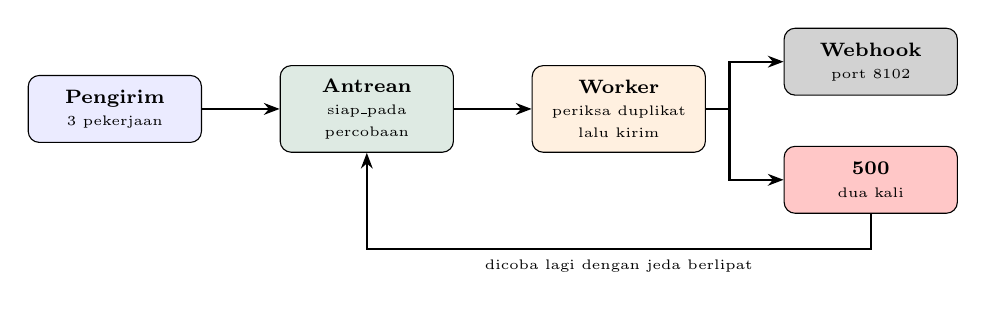
\begin{tikzpicture}[
    font=\scriptsize,
    kotak/.style={draw, rounded corners, minimum height=0.85cm,
                  minimum width=2.2cm, align=center, font=\scriptsize\bfseries},
    panah/.style={-{Stealth[length=2mm]}, thick}
  ]
    \node[kotak, fill=blue!8] (kirim) at (0,0) {Pengirim\\{\tiny\mdseries 3 pekerjaan}};
    \node[kotak, fill=praditagreen!15, minimum height=1.1cm] (antrean) at (3.2,0) {Antrean\\{\tiny\mdseries siap\_pada}\\{\tiny\mdseries percobaan}};
    \node[kotak, fill=orange!12, minimum height=1.1cm] (worker) at (6.4,0) {Worker\\{\tiny\mdseries periksa duplikat}\\{\tiny\mdseries lalu kirim}};
    \node[kotak, fill=gray!35] (webhook) at (9.6,0.6) {Webhook\\{\tiny\mdseries port 8102}};
    \node[kotak, fill=red!22] (gagal) at (9.6,-0.9) {500\\{\tiny\mdseries dua kali}};

    \draw[panah] (kirim) -- (antrean);
    \draw[panah] (antrean) -- (worker);
    \draw[panah] (worker.east) -- ++(0.3,0) |- (webhook.west);
    \draw[panah] (worker.east) -- ++(0.3,0) |- (gagal.west);
    \draw[panah] (gagal.south) -- ++(0,-0.45) -| node[font=\tiny, below, pos=0.25] {dicoba lagi dengan jeda berlipat} (antrean.south);
  \end{tikzpicture}
  \vspace{2pt}
  {\small Analoginya loket surat: mahasiswa menerima tanda terima lalu
  pulang, dan petugas di belakang mengerjakan berkasnya menurut urutan.}
\end{frame}

\begin{frame}[fragile]{{\Large Pekerjaan yang Diambil Tidak Langsung Hilang}}
  \vspace{2pt}
\begin{lstlisting}[style=PythonStyle]
  keadaan = muat()
  for pesan in keadaan["pesan"]:
    if pesan["siap_pada"] <= sekarang:
      pesan["percobaan"] += 1
      pesan["siap_pada"] = sekarang + jeda_backoff(pesan["percobaan"])
      simpan(keadaan)
      return dict(pesan)
  return None
\end{lstlisting}
  \vspace{2pt}
  {\small Pergeseran waktu siap itu disebut \textit{visibility timeout}.
  Akibatnya dua: pekerjaan tidak hilang ketika \textit{worker}-nya mati, dan
  pekerjaan dapat dikerjakan dua kali.}
\end{frame}

\section{Retry dan Exponential Backoff}

\begin{frame}{\hfill}
  \centering
  \Huge{\textbf{Retry dan Exponential Backoff}}
\end{frame}

\begin{frame}{{\Large Enam Percobaan pada Satu Daur, Diukur}}
  \vspace{6pt}
  \centering
  {\footnotesize
  \begin{tabularx}{\textwidth}{llYl}
    \hline
    \textbf{Pekerjaan} & \textbf{Ke} & \textbf{Hasil} & \textbf{Detik} \\
    \hline
    \texttt{kerja-0001} & 1 & terkirim dan di-\textit{ack} & 0,01 \\
    \hline
    \texttt{kerja-0002} & 1 & gagal, \textit{webhook} 500 & 0,01 \\
    \hline
    \texttt{kerja-0003} & 1 & terkirim, mati sebelum \textit{ack} & 0,01 \\
    \hline
    \texttt{kerja-0002} & 2 & gagal, \textit{webhook} 500 & 0,51 \\
    \hline
    \texttt{kerja-0003} & 2 & duplikat ditahan & 0,51 \\
    \hline
    \texttt{kerja-0002} & 3 & terkirim dan di-\textit{ack} & 1,52 \\
    \hline
  \end{tabularx}}
  \vspace{6pt}
  {\small Jeda dasarnya 0,5 detik: percobaan kedua 0,5 detik sesudah yang
  pertama, dan yang ketiga 1,0 detik sesudah yang kedua.}
\end{frame}

\begin{frame}[fragile]{{\Large Satu Baris yang Menahan Banjir Percobaan}}
  \vspace{2pt}
\begin{lstlisting}[style=PythonStyle]
def jeda_backoff(percobaan):
  """Menghitung jeda sebelum percobaan berikutnya, berlipat dua tiap kali.

  Jeda yang berlipat menahan worker dari membanjiri tujuan yang sedang
  bermasalah. Percobaan pertama memakai jeda dasar, yang kedua dua kali,
  yang ketiga empat kali, dan seterusnya.
  """
  return JEDA_DASAR_DETIK * (2 ** max(0, percobaan - 1))
\end{lstlisting}
  \vspace{2pt}
  {\small Pekerjaan yang tetap gagal sesudah batas percobaan pantas
  dipindahkan ke \textit{dead letter queue}, agar antreannya tidak tersumbat
  satu pekerjaan yang tidak akan pernah berhasil.}
\end{frame}

\section{Consumer Idempoten dan At-Least-Once}

\begin{frame}{\hfill}
  \centering
  \Huge{\textbf{Consumer Idempoten\\dan At-Least-Once}}
\end{frame}

\begin{frame}{{\Large Enam Percobaan, Lima Pengiriman Tiba}}
  \vspace{6pt}
  \centering
  {\footnotesize
  \begin{tabularx}{\textwidth}{Ylll}
    \hline
    \textbf{Pekerjaan} & \textbf{Percobaan} & \textbf{Tiba} & \textbf{Akibat di tujuan} \\
    \hline
    \texttt{kerja-0001}, lancar & 1 & 1 & satu kali \\
    \hline
    \texttt{kerja-0002}, ditolak dua kali & 3 & 3 & satu kali, pada percobaan ketiga \\
    \hline
    \texttt{kerja-0003}, \textit{worker} mati & 2 & 1 & satu kali \\
    \hline
    \textbf{Jumlah} & \textbf{6} & \textbf{5} & \textbf{3 pekerjaan tuntas} \\
    \hline
  \end{tabularx}}
  \vspace{6pt}
  {\small Baris ketiga memuat hasil yang dicari: dikirim dua kali oleh
  \textit{worker}, tiba sekali di \textit{webhook}, karena pengiriman kedua
  berhenti di pemeriksaan duplikat.}
\end{frame}

\begin{frame}[fragile]{{\Large Urutannya yang Menentukan}}
  \vspace{2pt}
\begin{lstlisting}[style=PythonStyle]
  if antrean.sudah_diproses(pesan["id"]):
    antrean.selesai(pesan["id"])
    return "duplikat ditahan"
  status = kirim_webhook(pesan)
  if status != 200:
    return f"gagal, webhook {status}, dicoba lagi nanti"
  antrean.tandai_diproses(pesan["id"])
\end{lstlisting}
  \vspace{2pt}
  {\small Pemeriksaan duplikat diletakkan sebelum pengiriman, karena di
  sanalah duplikat masih dapat ditahan tanpa akibat. Kuncinya id pekerjaan
  yang tetap, bukan id yang dibuat ulang tiap percobaan.}
\end{frame}

\section{Scheduled Job dan Eventual Consistency}

\begin{frame}{\hfill}
  \centering
  \Huge{\textbf{Scheduled Job dan\\Eventual Consistency}}
\end{frame}

\begin{frame}{{\Large Kedua Sisi Akan Sama, Tetapi Tidak Sekarang}}
  \vspace{6pt}
  \centering
  {\footnotesize
  \begin{tabularx}{\textwidth}{lYY}
    \hline
    \textbf{Detik} & \textbf{Sistem kita} & \textbf{Tujuan \textit{webhook}} \\
    \hline
    0,00 & tiga pekerjaan diterima & belum menerima apa pun \\
    \hline
    0,01 & dua tuntas, satu gagal & \texttt{kerja-0001} dan \texttt{kerja-0003} \\
    \hline
    0,51 & duplikat ditahan & masih belum tahu \texttt{kerja-0002} \\
    \hline
    1,52 & tiga tuntas & ketiganya sudah diterima \\
    \hline
  \end{tabularx}}
  \vspace{6pt}
  {\small Dua akibat praktisnya: tampilan tidak boleh berjanji lebih
  daripada yang sudah terjadi, dan jarak waktunya harus dipantau, karena
  antrean yang menumpuk tidak terlihat pada halaman mana pun.}
\end{frame}

\section{Persiapan Latihan}

\begin{frame}{\hfill}
  \centering
  \Huge{\textbf{Persiapan Latihan}}
\end{frame}

\begin{frame}[fragile]{{\Large Tiga Layanan, Urutannya Berpengaruh}}
  \vspace{2pt}
\begin{lstlisting}[language=bash]
cd sources/chapter13
python3 aplikasi.py &
python3 webhook.py &
python3 websocket.py &

# Keluarannya:
# Melayani di http://127.0.0.1:8100/sse dan /polling
# Webhook di http://127.0.0.1:8102/webhook, dua percobaan pertama ditolak
# WebSocket di ws://127.0.0.1:8101/
\end{lstlisting}
  \vspace{2pt}
  {\small \texttt{websocket.py} mengikuti aliran SSE aplikasi, jadi
  dinyalakan sesudahnya. Hanya Python 3, tanpa pustaka tambahan.}
\end{frame}

\section{Latihan 1 dan 2}

\begin{frame}{\hfill}
  \centering
  \Huge{\textbf{Latihan 1 dan 2:\\Transport dan Jeda Polling}}
\end{frame}

\begin{frame}[fragile]{{\Large Mengukur Ketiga Transport}}
  \vspace{2pt}
\begin{lstlisting}[language=bash]
python3 ukur-transport.py

# Keluarannya:
#   Transport   Peristiwa  Tengah ms  Tertinggi     Byte  Permintaan
#   polling            10      199.8      202.0      639          11
#   sse                10        1.8        2.0      400           1
#   websocket          10        1.9        2.1      490           1
\end{lstlisting}
  \vspace{2pt}
  {\small Lalu ubah \texttt{JEDA\_POLLING\_DETIK} menjadi 0,1 dan 1,0.
  Terukur: 3,3 ms dengan 31 permintaan, lalu 700,1 ms dengan 11 permintaan.}
\end{frame}

\section{Latihan 3 dan 4}

\begin{frame}{\hfill}
  \centering
  \Huge{\textbf{Latihan 3 dan 4:\\Retry dan Duplikat}}
\end{frame}

\begin{frame}[fragile]{{\Large Satu Daur Antrean dari Ujung ke Ujung}}
  \vspace{2pt}
\begin{lstlisting}[language=bash]
python3 ukur-antrean.py | tail -3

# Keluarannya:
#   Percobaan worker: 6, pengiriman tiba: 5, pekerjaan tersisa: 0,
#   ditandai diproses: 3
\end{lstlisting}
  \vspace{4pt}
  {\small Lalu matikan pemeriksaan duplikat di \texttt{worker.py}, jalankan
  ulang, dan catat jumlah pengiriman yang tiba sekarang. Pulihkan kembali
  sesudahnya.}
\end{frame}

\section{Ringkasan}

\begin{frame}{\hfill}
  \centering
  \Huge{\textbf{Ringkasan}}
\end{frame}

\begin{frame}{{\Large Ringkasan}}
  \vspace{8pt}
  \begin{itemize}
    \item \textit{Polling} jeda 0,5 detik menyerahkan peristiwa dalam 199,8
          ms dengan 11 permintaan. SSE 1,8 ms dan WebSocket 1,9 ms, keduanya
          lewat satu sambungan.
    \item Pilihan di antara keduanya bukan soal angka: SSE satu arah dan
          menyambung ulang sendiri, WebSocket dua arah tetapi diurus sendiri.
    \item Antrean menggeser waktu siap tiap pekerjaan yang diambil, sehingga
          pekerjaan tidak hilang, dengan ganti dapat terkirim lebih dari
          sekali.
    \item Enam percobaan menghasilkan lima pengiriman tiba dan tiga pekerjaan
          tuntas. Jeda \textit{retry} terukur 0,5 lalu 1,0 detik.
    \item Antrean hanya menjamin pekerjaan tidak hilang. Jaminan akibatnya
          tidak terjadi dua kali hanya dapat ditegakkan \textit{consumer}.
  \end{itemize}
\end{frame}

\end{document}
